\documentclass[10pt,journal,compsoc]{IEEEtran}

\usepackage[utf8]{inputenc}
\usepackage{amsmath,amssymb,amsfonts}
\usepackage{graphicx}
\usepackage{booktabs}
\usepackage{microtype}
\usepackage{xcolor}
\usepackage{hyperref}
\usepackage{cite}
\usepackage{subcaption}
\usepackage{listings}

% Figures are resolved from results/figures/ (this file lives in results/reports/).
\graphicspath{{../figures/}}

\hypersetup{
    colorlinks=true,
    linkcolor=blue,
    citecolor=blue,
    urlcolor=blue
}

% The four multi-panel figure* floats are taller than half the text height,
% so some pages cannot be stretched to exactly \textheight.  \raggedbottom
% lets those pages end short instead of reporting
% "Underfull \vbox (badness 10000) ... while \output is active".
% (Remove this line if IEEE-style flush-bottom pages are required.)
\raggedbottom

\begin{document}

\title{Deadlock-Free Flow Control in 1D-Ring Networks: \\ Escape Virtual Channels and Bubble Flow Control}

\author{}

\IEEEtitleabstractindextext{%
\begin{abstract}
Ring topologies (1D-Tori) are widely deployed in commercial multicore processors and chiplet-based architectures due to their low router radix, simple wiring, and minimal silicon footprint. However, when paired with high-performance minimal (shortest-path) routing, circular physical channels inevitably introduce cyclic channel dependencies, leading to catastrophic routing deadlocks under moderate-to-high traffic loads. In this project, we design, implement, and evaluate two representative deadlock-avoidance flow control paradigms in gem5/Garnet 3.0 on a 16-node bidirectional Ring network: (1) \textit{Escape Virtual Channels}, which partitions virtual channels into an adaptive subnetwork and an acyclic Dateline-cut escape subnetwork based on Duato's Theorem, dynamically falling back to escape channels upon congestion; and (2) \textit{Bubble Flow Control}, which enforces capacity-invariant regulation via dual hardware gates (Injection Gate and Ring-Entry Gate) to perpetually maintain traveling empty buffer slots (bubbles) in each ring direction. Extensive synthetic evaluations across uniform random, bit-complement, and bit-reverse traffic patterns validate that both mechanisms successfully eliminate routing deadlocks, dramatically extending the network saturation threshold while revealing critical architectural trade-offs between hardware complexity, latency, and peak throughput.
\end{abstract}}

\maketitle
\IEEEdisplaynontitleabstractindextext
\IEEEpeerreviewmaketitle

% =========================================================================
% SECTION 1: INTRODUCTION & MOTIVATION
% =========================================================================
\section{Introduction and Motivation}
\IEEEPARstart{A}{s} semiconductor technology integrates tens to hundreds of heterogeneous processing cores onto a single die or across multiple chiplets, the on-chip interconnect (Network-on-Chip, NoC) becomes the paramount determinant of overall system latency, throughput, and energy efficiency. Among various network topologies, the 1D-Ring (1D-Torus) architecture represents a prevalent commercial design point (e.g., utilized in Intel Xeon processors) due to its minimal router degree ($k=3$), localized point-to-point links, and low implementation overhead.

In Lab 3, we constructed a 16-node bidirectional Ring topology with a minimal (shortest-path) routing algorithm. While minimal routing minimizes zero-load hop count and transmission latency, it introduces a severe architectural hazard: \textbf{cyclic channel dependencies}~\cite{dally1987deadlock}. Because a Ring forms a closed physical loop:
\begin{equation}
\text{Router } 0 \to 1 \to \dots \to 15 \to 0
\end{equation}
simultaneous bidirectional or unidirectional packet forwarding can cause packets to fill all input buffers along the ring. Each packet holds its current buffer while requesting a downstream buffer occupied by the next packet, creating an inescapable circular wait condition (Coffman condition)~\cite{coffman1971deadlock}. Under baseline minimal routing, the network deadlocks prematurely (at injection rates as low as $0.04$ with a single VC under uniform random traffic, and $0.075$ under bit-reverse), causing packet delivery to freeze and triggering fatal simulation aborts.

To resolve this fundamental dilemma, Lab 4 investigates two foundational flow-control and deadlock-avoidance methodologies:
\begin{enumerate}
    \item \textbf{Escape Virtual Channels}: Based on Duato's Theorem, we segment the virtual channel (VC) resources into adaptive VCs (for low-latency shortest-path routing) and escape VCs (strictly constrained to an acyclic Dateline routing path). Blocked packets dynamically fall back to the escape subnetwork, guaranteeing forward progress.
    \item \textbf{Bubble Flow Control}: Rather than reserving dedicated escape channels, Bubble flow control preserves an invariant: each ring direction must permanently maintain at least one unoccupied buffer slot (a ``bubble''). By regulating local injection and ring entry through dual hardware gates, circular buffer exhaustion is provably eliminated.
\end{enumerate}

This report documents the architectural design, gem5/Garnet microarchitectural implementation, empirical benchmarking, and comparative analysis of both techniques.

% =========================================================================
% SECTION 2: ARCHITECTURE & BASELINE SYSTEM
% =========================================================================
\section{Architecture and Baseline System}

\subsection{16-Node Bidirectional Ring Topology}
The underlying physical network comprises $N=16$ routers (labeled $0$ through $15$) interconnected in a bidirectional 1D-Torus. Each router features three bidirectional ports:
\begin{itemize}
    \item \textbf{Local Port}: Interfaces directly with the local Network Interface (NI) for packet injection and ejection.
    \item \textbf{Right Port (Clockwise / East)}: Forwarding channel along $0 \to 1 \to 2 \to \dots \to 15 \to 0$.
    \item \textbf{Left Port (Counter-Clockwise / West)}: Forwarding channel along $0 \to 15 \to 14 \to \dots \to 1 \to 0$.
\end{itemize}

\subsection{Shortest-Path Minimal Routing Algorithm}
For a packet originating at source router $s$ destined for destination router $d$, the minimal clockwise distance $dist_{\text{cw}}$ and counter-clockwise distance $dist_{\text{ccw}}$ are calculated as:
\begin{align}
dist_{\text{cw}} &= (d - s + N) \pmod{N} \\
dist_{\text{ccw}} &= (s - d + N) \pmod{N}
\end{align}

The routing function selects the direction with the minimum hop distance:
\begin{equation}
\text{Outport} = \begin{cases} 
\text{Right (Clockwise)}, & \text{if } dist_{\text{cw}} \le dist_{\text{ccw}} \\
\text{Left (Counter-Clockwise)}, & \text{if } dist_{\text{cw}} > dist_{\text{ccw}}
\end{cases}
\end{equation}

\noindent \textbf{Tie-Breaking Policy (``Right if tie'')}: For diametrically opposite nodes where $dist_{\text{cw}} = dist_{\text{ccw}} = 8$ (e.g., node $0$ transmitting to node $8$), the algorithm deterministically selects the \textit{Right} port ($<=$ condition). While mathematically optimal in distance, this policy allows circular channel dependency chains to close in both directions, making deadlock inevitable when buffers saturate.

% =========================================================================
% SECTION 3: IMPLEMENTATION - ESCAPE VIRTUAL CHANNELS
% =========================================================================
\section{Implementation: Escape Virtual Channels}

\subsection{Theoretical Foundation (Duato's Theorem)}
Duato's Theorem~\cite{duato1993new} proves that a routing algorithm containing cycles in its Channel Dependency Graph (CDG) remains deadlock-free if and only if there exists a connected subnetwork whose CDG is strictly acyclic, and packets are always granted access to this subnetwork when blocked in the adaptive channels.

We partition the VCs per virtual network into two classes:
\begin{equation}
VCs = \underbrace{\{0, \dots, E-1\}}_{\text{Escape VCs}} \cup \underbrace{\{E, \dots, V-1\}}_{\text{Adaptive VCs}}
\end{equation}
where $E = \texttt{--escape-vc-per-vnet}$ ($E \ge 1$) specifies the number of escape channels reserved at the lowest indices of each virtual network.

\subsection{Acyclic Dateline Routing Function}
To render the escape subnetwork strictly acyclic, we define a virtual \textbf{Dateline} between Router $0$ and Router $15$~\cite{dally1987deadlock}. In the escape channels, packets are forbidden from crossing the Dateline:
\begin{equation}
\text{Escape Outport} = \begin{cases}
\text{Right}, & \text{if } d \ge s \\
\text{Left}, & \text{if } d < s
\end{cases}
\end{equation}
The boundary case $d=s$ cannot occur for a flit that still needs routing (it is already at its destination and is ejected); the implementation resolves the comparison as $d \ge s$ and would select \texttt{Right}.
By banning wrap-around transitions ($0 \to 15$ westward or $15 \to 0$ eastward in escape channels), the circular channel dependency is cleanly severed. The escape channels form a directed acyclic graph (DAG) topologically equivalent to a linear bidirectional bus, guaranteeing finite-time packet drain.

\subsection{Microarchitectural Pipeline in Garnet}
The complete routing and arbitration pipeline for Escape VCs is implemented across five coordinated stages (see Figure~\ref{fig:escape_vc_pipeline}):

\begin{enumerate}
    \item \textbf{Route Precomputation (\texttt{InputUnit.cc})}:
    Upon the arrival of a packet head flit at an input VC, the router computes \textit{both} the minimal adaptive route and the acyclic escape route simultaneously, storing them via \texttt{grant\_outport\_adaptive()} and \texttt{grant\_outport\_escape()}.
    
    \item \textbf{Route Computation (\texttt{RoutingUnit.cc})}:
    \texttt{outportComputeRing()} calculates the shortest-path direction, while \texttt{outportComputeRingEscape()} determines the non-wrapping Dateline direction.
    
    \item \textbf{Route and VC Class Selection (\texttt{SwitchAllocator.cc})}:
    During the switch allocation stage (SA-I), the allocator arbitrates between classes:
    \begin{itemize}
        \item If the flit already occupies an Escape VC, it is strictly bound to the escape path (\texttt{vc\_class = ESCAPE\_VC\_}).
        \item If the flit occupies an Adaptive VC, it first attempts to reserve a free Adaptive VC on its optimal adaptive outport.
        \item \textbf{Dynamic Fallback}: If all adaptive VCs on the optimal outport are occupied, but an Escape VC on the escape outport is available, the flit dynamically falls back to the escape class.
        \item Otherwise, the flit stalls and waits.
    \end{itemize}
    
    \item \textbf{Output VC Allocation (\texttt{OutputUnit.cc})}:
    \texttt{select\_free\_vc()} filters candidate output channels strictly within the chosen VC class, reserving the allocated channel for switch traversal.
    
    \item \textbf{Statistics Tracking (\texttt{SwitchAllocator.cc} / \texttt{Router.cc})}:
    Every head flit whose output VC is allocated from the escape class increments the counter
    \texttt{m\_escaped\_flits} in \texttt{SwitchAllocator::arbitrate\_outports()} (one count per escape-class output-VC allocation, including the final ejection),
    so escape subnetwork utilization is quantified; the per-router \texttt{escaped\_flits} statistic is then
    registered and exported in \texttt{Router.cc}, where \texttt{Router::collateStats()} reads the counter
    via \texttt{switchAllocator.get\_escaped\_flits()}.
\end{enumerate}

% -------------------------------------------------------------------------
% PLACEHOLDER: FIGURE 1 (Escape VC Pipeline from PPT Slide 3/4)
% -------------------------------------------------------------------------
\begin{figure}[t]
\centering
% =========================================================================
% TODO [USER INSERTION]: Insert Escape VC Pipeline Diagram (from PPT Slides 3 & 4)
% Example: \includegraphics[width=0.95\linewidth]{figures/escape_vc_pipeline.png}
% =========================================================================
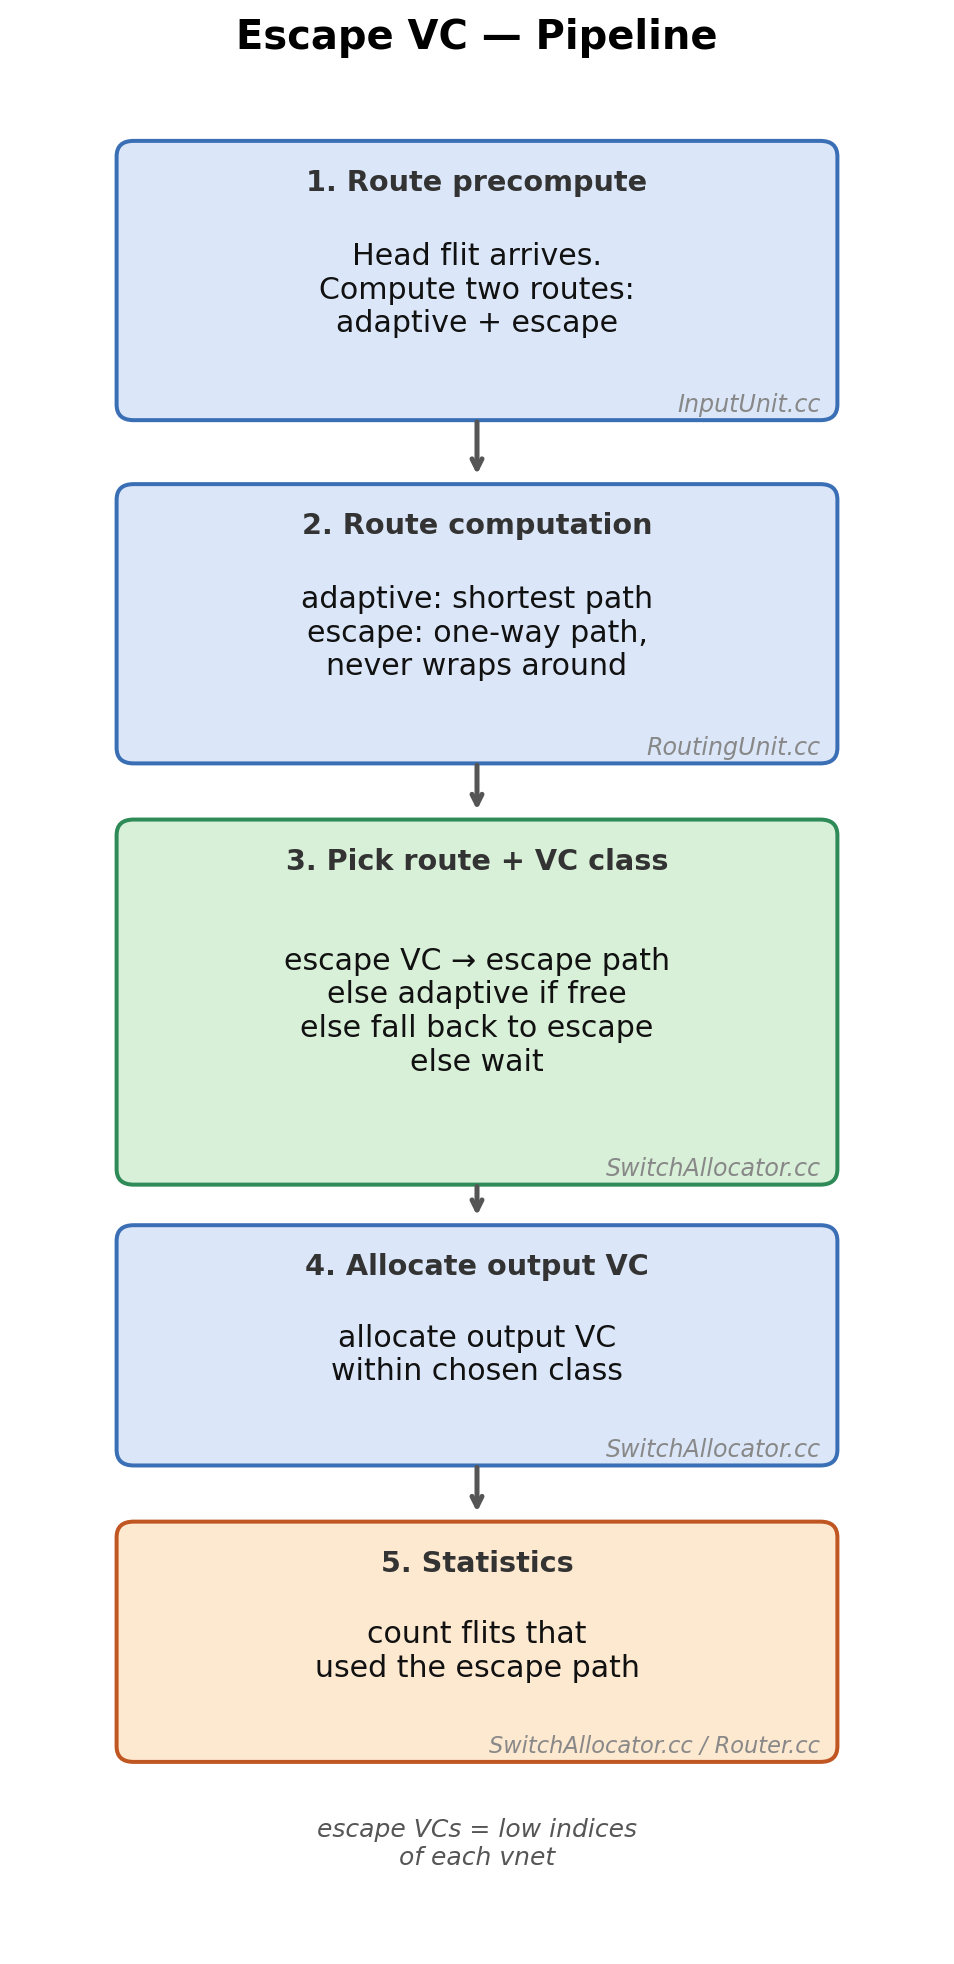
\includegraphics[width=0.95\linewidth]{impl_escape_vc_flow.png}
% \framebox[\linewidth]{\parbox{0.9\linewidth}{\centering \vspace{2.5cm} \textbf{[Figure 1 Placeholder: Escape VC Pipeline Architecture]} \\ \small (Insert diagram from PPT Slides 3 \& 4: Route Precompute $\to$ RoutingUnit $\to$ Pick Route/VC Class $\to$ Allocate Output VC $\to$ Statistics) \vspace{2.5cm}}}
\caption{Escape Virtual Channel microarchitectural pipeline in Garnet 3.0, illustrating concurrent route precomputation, adaptive-to-escape dynamic fallback in Switch Allocation, and class-aware output VC assignment.}
\label{fig:escape_vc_pipeline}
\end{figure}

% =========================================================================
% SECTION 4: IMPLEMENTATION - BUBBLE FLOW CONTROL
% =========================================================================
\section{Implementation: Bubble Flow Control}

\subsection{Capacity-Invariant Bubble Principle}
Bubble flow control~\cite{puente1999bubble} eliminates routing deadlocks without allocating dedicated physical escape channels or enforcing non-minimal routing detours. Its mathematical foundation rests on a simple capacity invariant:
\begin{equation}
\mathcal{N}_{\text{occ}}(\mathcal{D}) \le \mathcal{N}_{\text{total}}(\mathcal{D}) - B_{\text{min}}
\end{equation}
where $\mathcal{N}_{\text{occ}}(\mathcal{D})$ and $\mathcal{N}_{\text{total}}(\mathcal{D})$ denote the occupied and total buffer slots in ring direction $\mathcal{D}$, and $B_{\text{min}} \ge 1$ represents the mandatory number of unallocated buffer slots (the ``bubble'').

\textbf{Forwarding Conservation}: In a ring network, an in-flight packet traversing from Router $i$ to Router $i+1$ occupies a downstream buffer while simultaneously vacating an upstream buffer. The net change in ring buffer occupancy is zero. Therefore, \textit{ring forwarding never consumes a bubble}. 

\textbf{Injection Criticality}: Only local packet injection (from the network interface into the ring) increases total ring occupancy by $+1$. If injection is permitted unchecked, all buffers along a ring direction can fill, extinguishing the traveling bubble and causing immediate circular deadlock.

\subsection{Dual-Gate Microarchitecture}
To perpetually sustain traveling bubbles, we introduce two hierarchical hardware gating mechanisms (see Figure~\ref{fig:bubble_gates}):

\begin{enumerate}
    \item \textbf{Gate 1: Injection Gate (\texttt{NetworkInterface.cc})}:
    Before injecting a newly packetized flit into the router, the network interface interrogates the attached router's ring input ports. If the total number of idle ring VCs across both directions falls below the injection threshold:
    \begin{equation}
    N_{\text{idle, total}} < \theta_{\text{inject}} \quad (\text{where } \theta_{\text{inject}} = 2)
    \end{equation}
    the NI refuses injection and retains the packet in its injection FIFO queue. This gate provides global ring throttling and operates for all VC configurations, including single-VC networks ($VCs=1$).

    \item \textbf{Gate 2: Ring-Entry Gate (\texttt{SwitchAllocator.cc})}:
    For multi-VC networks ($VCs \ge 2$), packets at the router's \texttt{Local} inport requesting switch traversal into a ring outport (Right or Left) are subjected to a directional check:
    \begin{equation}
    N_{\text{idle, direction}} < \theta_{\text{enter}} \quad (\text{where } \theta_{\text{enter}} = 2)
    \end{equation}
    If the targeted ring direction does not possess at least two idle VCs, local ring entry is blocked. Crucially, packets already in transit within the ring (e.g., Right-in to Right-out) completely bypass Gate 2, ensuring ring-forwarding traffic maintains absolute priority over new entrants.
\end{enumerate}

% -------------------------------------------------------------------------
% PLACEHOLDER: FIGURE 2 (Bubble Dual Gates from PPT Slide 5)
% -------------------------------------------------------------------------
\begin{figure}[t]
\centering
% =========================================================================
% TODO [USER INSERTION]: Insert Bubble Dual Gates Diagram (from PPT Slide 5)
% Example: \includegraphics[width=0.95\linewidth]{figures/bubble_gates.png}
% =========================================================================
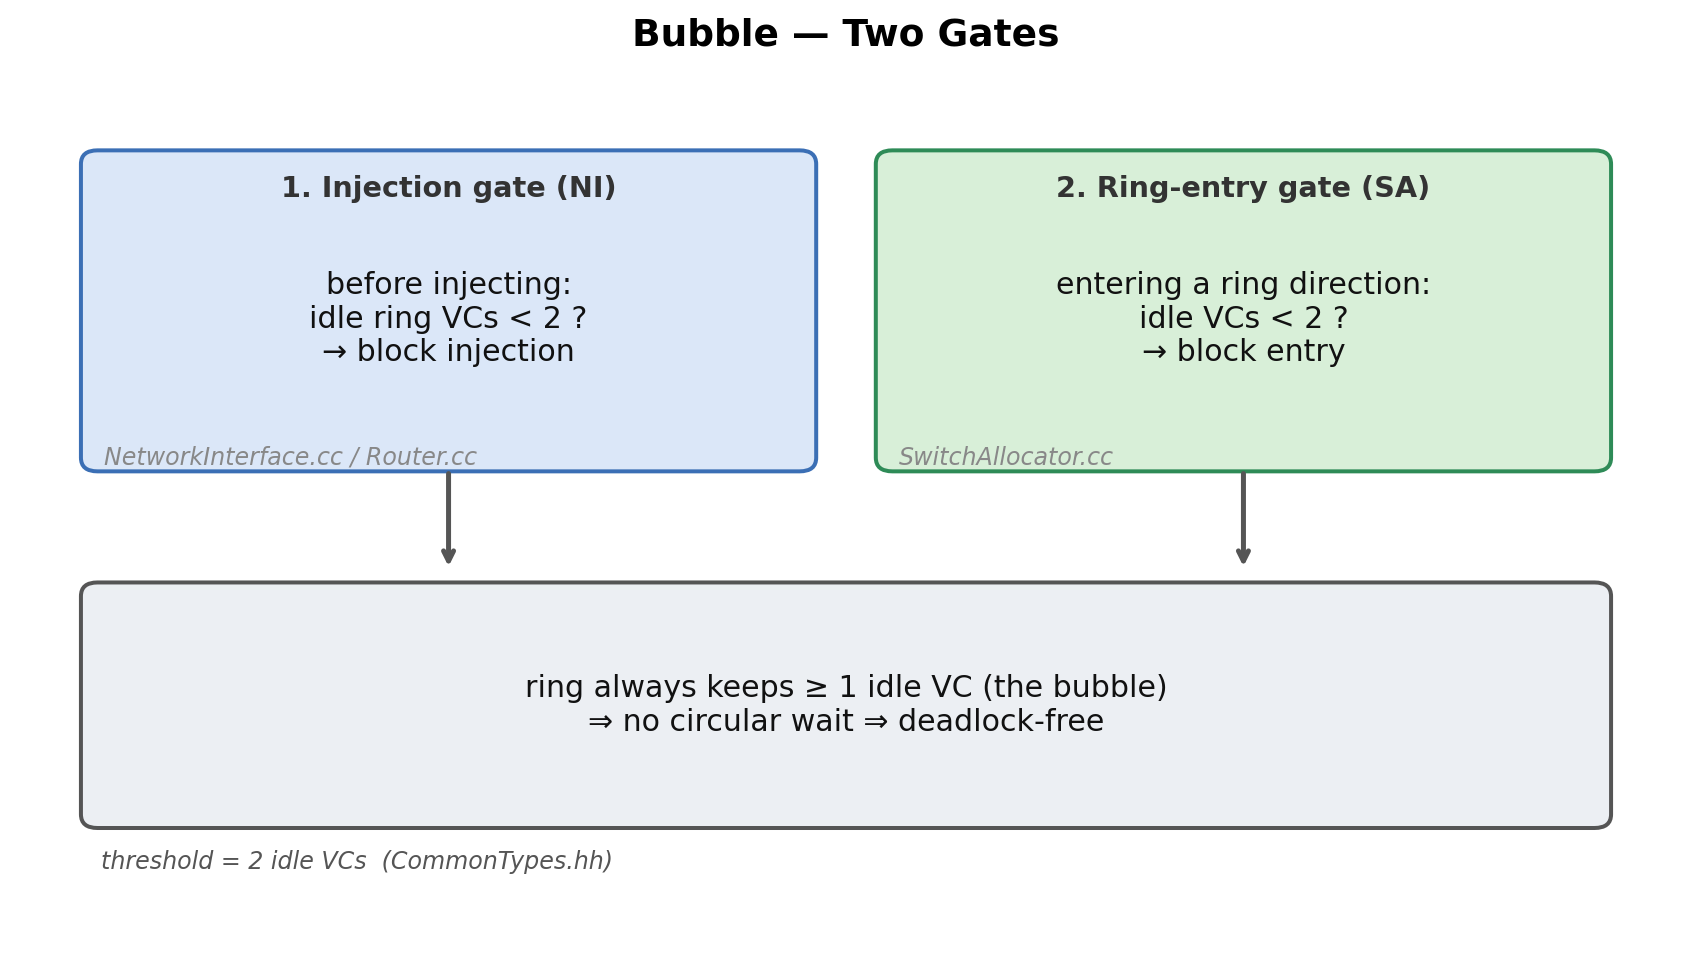
\includegraphics[width=0.95\linewidth]{impl_bubble_flow.png}
% \framebox[\linewidth]{\parbox{0.9\linewidth}{\centering \vspace{2.5cm} \textbf{[Figure 2 Placeholder: Bubble Flow Control Dual-Gate Architecture]} \\ \small (Insert diagram from PPT Slide 5: Gate 1 Injection Gate at NI + Gate 2 Ring-Entry Gate at SA $\to$ Sustained Ring Bubble $\to$ Deadlock Freedom) \vspace{2.5cm}}}
\caption{Bubble flow control dual-gate architecture. Gate 1 regulates injection from the network interface; Gate 2 regulates switch allocation from Local inport to Ring outports, guaranteeing the persistence of traveling bubbles.}
\label{fig:bubble_gates}
\end{figure}

% =========================================================================
% SECTION 5: EXPERIMENTAL EVALUATION
% =========================================================================
\section{Experimental Evaluation and Results}

\subsection{Experimental Methodology and Simulation Setup}
All experiments are conducted using the cycle-accurate gem5/Garnet 3.0~\cite{gem5} standalone network simulator configured with a 16-node bidirectional Ring topology ($N=16$, 1-cycle router latency, 1-cycle link latency, 128-bit link width, 1\,GHz clock frequency). Simulations run for 100,000 cycles with a deadlock detection threshold of 50,000 cycles. Synthetic single-flit control packets (\texttt{inj-vnet=0}) are injected over two rate grids: the bubble-flow-control campaign sweeps 15 fine-grained rates ($0.01 \sim 0.70$ packets/node/cycle), whereas the escape-VC sweep uses 7 coarser rates ($0.05$, $0.10$, $0.20$, $0.30$, $0.40$, $0.50$, $0.70$ packets/node/cycle). Since every packet is a single flit, ``flits'' and ``packets'' are interchangeable; note, however, that the escape-VC figures report \emph{network-level} throughput (flits/cycle summed over all $16$ nodes), while the bubble figures and Table~\ref{tab:comparison} report \emph{per-node} throughput (packets/node/cycle)---the two bases differ by a factor of~$16$. The bubble campaign uses three synthetic communication patterns:
\begin{itemize}
    \item \textbf{Uniform Random}: Destination nodes chosen uniformly at random among all $16$ nodes (the source itself may be drawn; such packets are absorbed locally without traversing the ring).
    \item \textbf{Bit-Complement}: Node $i$ transmits to $\sim i \pmod{16}$ (e.g., node 0 transmits to node 15), creating maximal bisection stress.
    \item \textbf{Bit-Reverse}: Node $i$ transmits to its bit-reversed address, generating localized traffic hotspots.
\end{itemize}

% -------------------------------------------------------------------------
% SUBSECTION 5.1: ESCAPE VC EVALUATION
% -------------------------------------------------------------------------
\subsection{Escape Virtual Channel Evaluation}
To evaluate Escape VCs, we fix the total buffer budget to $VCs=4$ and sweep the number of dedicated escape channels $E \in \{0, 1, 2, 3, 4\}$ under uniform random traffic, as detailed in PPT Slides 6 and 7.

% -------------------------------------------------------------------------
% PLACEHOLDER: FIGURE 3 (Escape VC 4-Subplot Evaluation from PPT Slide 7)
% -------------------------------------------------------------------------
\begin{figure*}[t]
\centering
% =========================================================================
% TODO [USER INSERTION]: Insert Escape VC 4-Panel Figure (from PPT Slide 7)
% Example: \includegraphics[width=0.98\linewidth]{figures/escape_vc_eval_4panel.png}
% =========================================================================
\includegraphics[width=0.95\linewidth]{escape_vc_eval.png}
% \framebox[\linewidth]{\parbox{0.95\linewidth}{\centering \vspace{4.0cm} \textbf{[Figure 3 Placeholder: Escape VC 4-Panel Evaluation (from PPT Slide 7)]} \\ \small (Insert 4-panel figure: Latency vs. Injection Rate, Accepted Throughput vs. Injection Rate, Escaped Flits vs. Injection Rate, and Average Hops vs. Injection Rate) \vspace{4.0cm}}}
\caption{Performance evaluation of Escape Virtual Channels on a 16-node Ring under uniform random traffic with $VCs=4$ across varying escape channels ($E \in \{0, 1, 2, 3, 4\}$). Subplots depict packet latency, accepted throughput, total escaped flits routed through Dateline escape channels, and average hop count. The throughput axis is network-level (flits/cycle); divide by $16$ to obtain packets/node/cycle.}
\label{fig:escape_vc_eval}
\end{figure*}

\textbf{Throughput and Deadlock Avoidance}: As shown in Figure~\ref{fig:escape_vc_eval}, the baseline unconstrained configuration ($E=0$, pure minimal adaptive) saturates normally up to rate $0.20$, accepting essentially all offered traffic ($3.19$ flits/cycle), but from rate $0.30$ onward every run deadlocks and the probe throughput collapses below $0.01$ flits/cycle. In stark contrast, allocating even a single escape channel ($E=1$) completely prevents deadlock across all injection rates up to $0.70$. However, because fallen-back packets then serialize onto one channel, $E=1$ sustains the lowest saturation throughput of all escape configurations ($\approx 1.15$ flits/cycle). The saturation throughput increases monotonically with the escape budget: $E=2$ sustains $\approx 1.92$ and $E=3$ $\approx 2.44$ flits/cycle, and the purely escape-routed configuration ($E=4$, all escape channels) reaches the highest value, $\approx 2.65$ flits/cycle, at the cost of longer (non-minimal) Dateline paths. All values in this subsection are network-level; dividing by the $16$ nodes yields the per-node throughputs used for the cross-technique comparison in Table~\ref{tab:comparison} ($E=1$: $\approx 0.07$, $E=2$: $\approx 0.12$, $E=3$: $\approx 0.15$, $E=4$: $\approx 0.17$ packets/node/cycle).

\textbf{Escaped Flits Dynamics}: The \textit{Escaped Flits vs. Injection Rate} curve demonstrates the adaptive-fallback behavior. The counter increments once per escape-class output-VC allocation (one count per hop on escape channels, plus the final ejection when a packet ejects from an escape VC), so it measures escape-channel utilization rather than a count of distinct packets. Even at the lowest injection rate ($0.05$), the escape class already accounts for roughly $30\%$ of all output-VC allocations under $E=1$ ($1.28 \times 10^5$ out of $\approx 4.3 \times 10^5$; the all-escape $E=4$ run, which records every allocation, totals $5.05 \times 10^5$). The counts peak around saturation at $\approx 3.7 \times 10^5$ ($E=1$) and $\approx 2.0 \times 10^6$ ($E=4$, rate $0.20$). This dynamic overflow drainage prevents adaptive channel saturation from escalating into circular deadlocks.

\textbf{Average Hop Count Overhead}: In the escape channels, Dateline-cut routing forbids ring wrap-around transitions, occasionally forcing packets to take the longer physical arc. Consequently, as the escape channel allocation increases from $E=1$ to $E=4$, the zero-load average hop count increases from $4.3$ to $5.3$ hops. However, under high loads, the average hop count across all operational configurations converges to $\approx 4.2 \sim 4.6$ hops as adaptive channels absorb the bulk of short-distance transfers.

% -------------------------------------------------------------------------
% SUBSECTION 5.2: BUBBLE FLOW CONTROL EVALUATION
% -------------------------------------------------------------------------
\subsection{Bubble Flow Control Evaluation Across Virtual Channel Depths}
Next, we evaluate Bubble flow control across virtual channel depths ($VCs=1, 2, 4$) under uniform random, bit-complement, and bit-reverse traffic patterns (corresponding to PPT Slides 8, 9, 10, and 11).

% -------------------------------------------------------------------------
% PLACEHOLDER: FIGURE 4 (VC=1 Bubble Evaluation from PPT Slide 9)
% -------------------------------------------------------------------------
\begin{figure*}[t]
\centering
% =========================================================================
% TODO [USER INSERTION]: Insert VC=1 Bubble Figure (from PPT Slide 9)
% Example: \includegraphics[width=0.98\linewidth]{figures/bubble_vc1_eval.png}
% =========================================================================
\includegraphics[width=0.95\linewidth]{bubble_vc1_eval.png}
% \framebox[\linewidth]{\parbox{0.95\linewidth}{\centering \vspace{3.5cm} \textbf{[Figure 4 Placeholder: Bubble Flow Control Evaluation with $VCs=1$ (from PPT Slide 9)]} \\ \small (Insert 3-row $\times$ 3-column figure for $VCs=1$ across Bit-Complement, Bit-Reverse, and Uniform Random traffic patterns) \vspace{3.5cm}}}
\caption{Evaluation of Bubble flow control with $VCs=1$ across Bit-Complement, Bit-Reverse, and Uniform Random traffic patterns. Subplots display latency, accepted throughput, and average hop count comparing the naive baseline (which deadlocks under uniform random and bit-reverse) against bubble control.}
\label{fig:bubble_vc1}
\end{figure*}

% -------------------------------------------------------------------------
% PLACEHOLDER: FIGURE 5 (VC=2 Bubble & Escape Evaluation from PPT Slide 10)
% -------------------------------------------------------------------------
\begin{figure*}[t]
\centering
% =========================================================================
% TODO [USER INSERTION]: Insert VC=2 Bubble Figure (from PPT Slide 10)
% Example: \includegraphics[width=0.98\linewidth]{figures/bubble_vc2_eval.png}
% =========================================================================
\includegraphics[width=0.95\linewidth]{bubble_vc2_eval.png}
% \framebox[\linewidth]{\parbox{0.95\linewidth}{\centering \vspace{3.5cm} \textbf{[Figure 5 Placeholder: Bubble vs. Escape VC Evaluation with $VCs=2$ (from PPT Slide 10)]} \\ \small (Insert 3-row $\times$ 3-column figure for $VCs=2$ comparing Naive, Bubble, and Escape VC [1 escape + 1 adaptive]) \vspace{3.5cm}}}
\caption{Evaluation of flow control techniques with $VCs=2$ across Bit-Complement, Bit-Reverse, and Uniform Random traffic patterns. Direct comparison between Naive Baseline, Bubble Flow Control, and Escape VC ($E=1$).}
\label{fig:bubble_vc2}
\end{figure*}

% -------------------------------------------------------------------------
% PLACEHOLDER: FIGURE 6 (VC=4 Bubble & Escape Evaluation from PPT Slide 11)
% -------------------------------------------------------------------------
\begin{figure*}[t]
\centering
% =========================================================================
% TODO [USER INSERTION]: Insert VC=4 Bubble Figure (from PPT Slide 11)
% Example: \includegraphics[width=0.98\linewidth]{figures/bubble_vc4_eval.png}
% =========================================================================
\includegraphics[width=0.95\linewidth]{bubble_vc4_eval.png}
% \framebox[\linewidth]{\parbox{0.95\linewidth}{\centering \vspace{3.5cm} \textbf{[Figure 6 Placeholder: Bubble vs. Escape VC Evaluation with $VCs=4$ (from PPT Slide 11)]} \\ \small (Insert 3-row $\times$ 3-column figure for $VCs=4$ comparing Naive, Bubble, and Escape VC [1 escape + 3 adaptive]) \vspace{3.5cm}}}
\caption{Evaluation of flow control techniques with $VCs=4$ across Bit-Complement, Bit-Reverse, and Uniform Random traffic patterns, highlighting high-load throughput saturation and latency stability.}
\label{fig:bubble_vc4}
\end{figure*}

\textbf{Single-VC Performance ($VCs=1$, Figure~\ref{fig:bubble_vc1})}: 
Under a single virtual channel, the naive minimal ring network deadlocks at low loads under uniform random (from rate $0.04$) and bit-reverse (from $0.075$) traffic; under bit-complement, however, it never deadlocks and merely saturates at $0.0625$ packets/node/cycle. Bubble flow control with Gate 1 eliminates every deadlock without any virtual channel support, but at a heavy throughput cost: only bit-complement keeps retiring packets at its saturation plateau ($0.0625$), while under uniform random the accepted throughput collapses from rate $0.05$ (below $3 \times 10^{-3}$, dropping to $54$ delivered flits per 100,000 cycles at rate $0.20$) and under bit-reverse from $0.075$. The ring is therefore deadlock-free but effectively starved, with un-admitted packets accumulating in the injection queues; no run triggers the deadlock detector during the entire 100,000-cycle execution.

\textbf{Dual-VC Performance ($VCs=2$, Figure~\ref{fig:bubble_vc2})}:
With $VCs=2$, the naive baseline continues to suffer catastrophic deadlocks under uniform random (from rate $0.10$) and bit-reverse (from $0.15$) traffic, while bit-complement never deadlocks. Both Bubble Flow Control and Escape VC ($E=1$, 1 escape + 1 adaptive) eliminate deadlocks. Bubble flow control reaches a smooth throughput saturation plateau at $0.15$ (uniform random) to $0.20$ (bit-reverse) packets/node/cycle. Escape VC shows a slightly \emph{higher} zero-load latency (e.g., $14.5$ vs.\ $12.9$ cycles under uniform random) because with only one adaptive VC some packets fall back to the longer Dateline route even at light load (zero-load hops $4.68$ vs.\ $3.96$), and it saturates at a substantially lower throughput ($0.061$ vs.\ $0.150$ packets/node/cycle under uniform random).

\textbf{Quad-VC Performance ($VCs=4$, Figure~\ref{fig:bubble_vc4})}:
At $VCs=4$, the baseline naive ring deadlocks at moderate injection rates (from $0.25$ under uniform random and $0.30$ under bit-reverse; bit-complement never deadlocks, saturating at $0.25$). Escape VC ($E=1$, 1 escape + 3 adaptive) eliminates deadlock, but the single escape channel becomes the throughput bottleneck: it saturates at only $0.072$ (uniform random), $0.244$ (bit-reverse) and $0.219$ (bit-complement) packets/node/cycle. Bubble flow control keeps routing fully minimal and achieves the highest saturation throughput among the three mechanisms under uniform random ($0.325$) and bit-reverse ($0.409$); under bit-complement it plateaus at $0.233$, slightly below the naive baseline ($0.250$)---the one pattern where the network is already deadlock-free on its own, so the bubble gates only reduce throughput.

% -------------------------------------------------------------------------
% SUBSECTION 5.3: ARCHITECTURAL TRADE-OFF ANALYSIS
% -------------------------------------------------------------------------
\subsection{Comparative Architectural Trade-Off Analysis}
Table~\ref{tab:comparison} synthesizes the qualitative and quantitative trade-offs between the evaluated deadlock-avoidance mechanisms.

\begin{table*}[t]
\centering
\caption{Architectural Comparison of Deadlock-Avoidance Flow Control Techniques on 16-Node Ring Network. All throughput entries are per-node (packets/node/cycle); the escape entries are converted from the network-level flits/cycle measurements of Figure~\ref{fig:escape_vc_eval} by dividing by the $16$ nodes.}
\label{tab:comparison}
\resizebox{\textwidth}{!}{%
\begin{tabular}{lcccc}
\toprule
\textbf{Metric / Attribute} &
\textbf{Baseline Ring} &
\textbf{Escape VC ($E=1$)} &
\textbf{Bubble Flow Control} &
\textbf{Pure Escape ($E=All$)} \\
\midrule
\textbf{Deadlock Freedom} &
\shortstack{No\\ (UR/BR deadlock)} &
\textbf{\shortstack{Yes\\ (Provably Acyclic)}} &
\textbf{\shortstack{Yes\\ (Capacity Invariant)}} &
\textbf{\shortstack{Yes\\ (Strict DAG)}} \\
\midrule
\textbf{Minimum Required VCs} &
1 &
\shortstack{2\\ (1 Escape + 1 Adaptive)} &
\textbf{\shortstack{1\\ (Operates on single VC)}} &
1 \\
\midrule
\textbf{Routing Adaptivity} &
Fully Minimal &
\textbf{\shortstack{Dynamic Adaptive\\ + Fallback}} &
Fully Minimal &
\shortstack{Non-adaptive\\ (Dateline)} \\
\midrule
\textbf{Hardware Overhead} &
Minimal &
\shortstack{Medium\\ (Dual Route + Class SA)} &
\textbf{\shortstack{Minimal\\ (Threshold Counters)}} &
\shortstack{Low\\ (Dateline Logic)} \\
\midrule
\textbf{Average Hop Count} &
\shortstack{Minimal\\ ($4.0$)} &
\shortstack{Slightly Inflated\\ ($4.3 \sim 4.7$)} &
\textbf{\shortstack{Minimal\\ ($4.0$)}} &
\shortstack{Inflated\\ ($5.3$)} \\
\midrule
\textbf{\shortstack[l]{Peak Saturation\\ Throughput}} &
\shortstack{Zero\\ (UR/BR deadlock)} &
\textbf{\shortstack{Low--Medium\\ ($0.06 \sim 0.24$)}} &
\textbf{\shortstack{Highest\\ ($0.33 \sim 0.41$ at $VCs=4$)}} &
\shortstack{Moderate\\ ($\approx 0.17$ at $VCs=4$)} \\
\midrule
\textbf{\shortstack[l]{Queueing Latency\\ under Overload}} &
\shortstack{N/A\\ (Frozen)} &
\shortstack{High\\ (Escape Channel Serialization)} &
\shortstack{High\\ (Admission Throttled)} &
High \\
\bottomrule
\end{tabular}%
}
\end{table*}

\begin{itemize}
    \item \textbf{Escape Virtual Channels} guarantee forward progress for any VC budget, but our experiments show that a single escape channel ($E=1$) serializes the fallen-back traffic and limits the saturation throughput to only $0.06 \sim 0.24$ packets/node/cycle. Reserving more escape VCs ($E=2,3$) or routing everything on the Dateline ($E=4$, $\approx 2.65$ flits/cycle network-level) restores throughput, at the cost of extra buffers and longer (non-minimal) paths.
    \item \textbf{Bubble Flow Control} achieves the highest saturation throughput under uniform random and bit-reverse whenever the router provides at least two VCs of slack ($0.33 \sim 0.41$ packets/node/cycle at $VCs=4$) while keeping routing fully minimal and requiring no extra buffers---only threshold-counting logic; the sole exception is bit-complement, where the naive ring is already deadlock-free and plateaus slightly higher ($0.250$ vs.\ $0.233$). On a single-VC router it eliminates deadlock but over-throttles the ring into starvation, so it is best suited to multi-VC, area-constrained designs.
\end{itemize}

\textbf{Why Bit-Complement Never Deadlocks}: The fact that the naive baseline survives bit-complement traffic at every VC count, while uniform random and bit-reverse eventually deadlock, is a property of the traffic pattern rather than of the flow control. Bit-complement pairs node $i$ with node $15-i$, and every complementary pair happens to lie within the same one of the two 8-node arcs $\{12,13,14,15,0,1,2,3\}$ (through the Dateline) and $\{4,5,6,7,8,9,10,11\}$: $(0,15)$, $(1,14)$, $\dots$, $(7,8)$. Consequently, no packet ever crosses the two ring edges $3$--$4$ and $11$--$12$ in either direction, and the input buffers of these four directed links stay permanently idle: the ring carries two natural ``holes'' and degenerates into two independent bidirectional lines. Since the two directions use disjoint buffers and, on a line, each per-direction wait-for chain is open (it cannot wrap around to close a cycle), no circular buffer dependency can form --- even a single VC per vnet suffices. This is precisely the invariant that bubble flow control enforces explicitly (keep at least one idle VC), except that here the traffic pattern provides it for free---which is why the baseline entry of Table~\ref{tab:comparison} scopes the deadlock to uniform random and bit-reverse. Those two patterns do traverse the cut edges, so their cyclic chains can close and deadlock occurs at low rates (as early as $0.04$ and $0.075$ packets/node/cycle at $VCs=1$).


% =========================================================================
% SECTION 6: CONCLUSION
% =========================================================================
\section{Conclusion}
This capstone project comprehensively addressed the critical routing deadlock problem inherent to minimal-routed 1D-Ring networks. By implementing and evaluating \textbf{Escape Virtual Channels} and \textbf{Bubble Flow Control} within gem5/Garnet 3.0, we demonstrated that routing deadlocks can be systematically eliminated through either topological channel decomposition (Duato's Theorem) or capacity-invariant admission regulation (Bubble Dual Gates). Our extensive benchmark sweeps across diverse synthetic traffic patterns highlight that Bubble Flow Control sustains the highest throughput once routers provide at least two VCs ($0.33 \sim 0.41$ packets/node/cycle at $VCs=4$), whereas Escape VCs guarantee progress for any VC budget but pay a throughput penalty unless several escape channels are reserved (a single escape channel saturates at only $0.06 \sim 0.24$ packets/node/cycle). These insights provide valuable architectural guidance for the design of scalable, deadlock-free interconnection networks in modern multicore and chiplet computing paradigms.

\begin{thebibliography}{1}

\bibitem{dally1987deadlock}
W.~J. Dally and C.~L. Seitz, ``Deadlock-free message routing in multiprocessor interconnection networks,'' \emph{IEEE Transactions on Computers}, vol.~C-36, no.~5, pp.~547--553, 1987.

\bibitem{coffman1971deadlock}
E.~G. Coffman, Jr., M.~J. Elphick, and A.~Shoshani, ``System deadlocks,'' \emph{ACM Computing Surveys}, vol.~3, no.~2, pp.~67--78, 1971.

\bibitem{duato1993new}
J.~Duato, ``A new theory of deadlock-free adaptive routing in wormhole networks,'' \emph{IEEE Transactions on Parallel and Distributed Systems}, vol.~4, no.~12, pp.~1320--1331, 1993.

\bibitem{puente1999bubble}
V.~Puente, R.~Beivide, J.~A. Gregorio, J.~M. Prellezo, J.~Duato, and C.~Izu, ``Adaptive bubble router: a design to improve performance in torus networks,'' in \emph{Proc.\ Int.\ Conf.\ on Parallel Processing (ICPP)}, 1999.

\bibitem{gem5}
N.~Binkert \emph{et al.}, ``The gem5 simulator,'' \emph{ACM SIGARCH Computer Architecture News}, vol.~39, no.~2, pp.~1--7, 2011.

\end{thebibliography}

\end{document}
